%Plantilla basada en "Template for Masters / Doctoral Thesis" (plantilla disponible en writeLaTex) que subió LaTeXTemplates.com

\documentclass[11pt]{book}
\usepackage[paperwidth=17cm, paperheight=22.5cm, bottom=2.5cm, right=2.5cm]{geometry}
\usepackage{amssymb,amsmath,amsthm} %paquete para símbolo matemáticos
\usepackage[spanish]{babel}
\usepackage[utf8]{inputenc} %Paquete para escribir acentos y otros símbolos directamente
\usepackage{enumerate}
\usepackage{graphicx}
%\usepackage{subfig} %para poner subfiguras
\graphicspath{{Img/}} %En qué carpeta están las imágenes
\usepackage[nottoc]{tocbibind}
\usepackage[pdftex,
            pdfauthor={NOMBRE DEL AUTOR},
            pdftitle={TÍTULO DE LA TESIS},
            pdfsubject={ÁREA DE LA TESIS},
            pdfkeywords={PALABRAS CLAVE},
            pdfproducer={Latex con hyperref},
            pdfcreator={pdflatex}]{hyperref}



\begin{document}

%----------------------------------------------------------------------------------------
%	COMANDOS PERSONALIZADOS
%----------------------------------------------------------------------------------------

%SI TU TESIS TIENE TEOREMAS Y DEMOSTRACIONES, PUEDES DESCOMENTAR Y USAR LOS SIGUIENTES COMANDOS

%\renewcommand{\proofname}{Demostración}
%\providecommand{\norm}[1]{\lVert#1\rVert} %Provee el comando para producir una norma.
%\providecommand{\innp}[1]{\langle#1\rangle} 
%\newcommand{\seno}{\mathrm{sen}}
%\newcommand{\diff}{\mathrm{d}}

%\newtheorem{teo}{Teorema}[section] 
%\newtheorem{cor}[teo]{Corolario}
%\newtheorem{lem}[teo]{Lema}

%\theoremstyle{definition}
%\newtheorem{dfn}[teo]{Definición}

%\theoremstyle{remark}
%\newtheorem{obs}[teo]{Observación}

%\allowdisplaybreaks


%----------------------------------------------------------------------------------------
%	PORTADA
%----------------------------------------------------------------------------------------

\title{TÍTULO DE LA TESIS} %Con este nombre se guardará el proyecto en writeLaTex

\begin{titlepage}
\begin{center}

\textsc{\Large Instituto Tecnológico Autónomo de México}\\[4em]

%Figura
\begin{figure}[h]
\begin{center}

\includegraphics{logo-ITAM_ch.jpg}
\end{center}
\end{figure}

\vspace{4em}

\textsc{\huge \textbf{TÍTULO DE LA TESIS}}\\[4em]

\textsc{\large Tesis}\\[1em]

\textsc{que para obtener el título de}\\[1em]

\textsc{TÍTULO  VAS A OBTENER}\\[1em]

\textsc{presenta}\\[1em]

\textsc{\Large AUTOR}\\[1em]

\textsc{\large Asesor: NOMBRE}

\end{center}

\vspace*{\fill}
\textsc{México, D.F. \hspace*{\fill} 2014}

\end{titlepage}


%----------------------------------------------------------------------------------------
%	DECLARACIÓN
%----------------------------------------------------------------------------------------

\thispagestyle{empty}
\vspace*{\fill}
\begingroup
``Con fundamento en los artículos 21 y 27 de la Ley Federal del Derecho de Autor y como titular de los derechos moral y patrimonial de la obra titulada ``\textbf{TÍTULO DE LA TESIS}'', otorgo de manera gratuita y permanente al Instituto Tecnológico Autónomo de México y a la Biblioteca Raúl Bailléres Jr., la autorización para que fijen la obra en cualquier medio, incluido el electrónico, y la divulguen entre sus usuarios, profesores, estudiantes o terceras personas, sin que pueda percibir por tal divulgación una contraprestación''.

\centering

\hspace{3em}

\textsc{AUTOR}

\vspace{5em}

\rule[1em]{20em}{0.5pt} % Línea para la fecha

\textsc{Fecha}
 
\vspace{8em}

\rule[1em]{20em}{0.5pt} % Línea para la firma

\textsc{Firma}

\endgroup
\vspace*{\fill}


%----------------------------------------------------------------------------------------
%	DEDICATORIA
%----------------------------------------------------------------------------------------

\pagestyle{empty}
\frontmatter

\chapter*{}
\begin{flushright}
\textit{DEDICATORIA}
\end{flushright}


%----------------------------------------------------------------------------------------
%	AGRADECIMIENTOS
%----------------------------------------------------------------------------------------

\chapter*{Agradecimientos}
%\markboth{AGRADECIMIENTOS23}{AGRADECIMIENTOS} % encabezado 

¡Muchas gracias a todos!


%----------------------------------------------------------------------------------------
%	PREFACIO
%----------------------------------------------------------------------------------------

\chapter*{Prefacio}

\pagestyle{plain}
%\markboth{PREFACIO23}{PREFACIO} % encabezado 

PUEDEN QUITAR ESTA PARTE


%----------------------------------------------------------------------------------------
%	TABLA DE CONTENIDOS
%---------------------------------------------------------------------------------------

\tableofcontents


%----------------------------------------------------------------------------------------
%	TESIS
%----------------------------------------------------------------------------------------
\mainmatter %empieza la numeración de las páginas
\pagestyle{headings}

%  Incluye los capítulos en el folder de capítulos

\chapter{Introducción}

\textbf{Antecedentes}

A partir del uso cada vez más cotidiano de chat como medio de comunicación han surgido un gran número de plataformas de mensajería instantánea. Actualmente algunas empresas, sobre todo en Asia, han visto un aumento sustancial en ventas al usar plataformas como Line o Wechat para acercarse a sus clientes. Estos sistemas y plataformas han ido evolucionando y sofisticando su uso. A grado tal ha llegado la adopción del chat que para algunas empresas es la base de venta para todos sus productos.

Por un lado, a partir de la compra de Whatsapp por Facebook, se ha visto en la empresa californiana un interés sobre el uso de su plataforma de mensajería instantánea, Messenger, como plataforma para el contacto de empresas en Occidente. 
Desde la convención de desarrolladores de Facebook (F8) en 2016, donde anunciaron la apertura de su API para Messenger, se ha visto un constante crecimiento en el número de personas y empresas que quieren aprovechar a la gran base de usuarios que Facebook pone a su alcance.

Además existen trabajos que han demostrado que la automatización de flujos de adquisición de clientes es benéfico para empresas que buscan aumentar su base de clientes y ofrecer productos innovadores \cite{makar2014automatic}. Se considera que hay dos componentes principalmente front-end y back-end.\cite{patil2017comparative} Existen actualmente varias formas de crear un agente de este tipo y se compararán aquí más adelante. 

Por otro lado, Resuelve es una empresa cuya misión es ayudar a las personas a solucionar problemas financieros. Cuenta con más de 6 años de experiencia y sucursales por toda la República Mexicana y Colombia. Además de aproximadamente 1,600 colaboradores  Cuenta con varias líneas de negocio. Resuelve tu deuda es una reparadora de deuda y la línea de negocio más grande de la familia Resuelve. Para la  adquisición de clientes, el equipo de marketing en Resuelve, ha encontrado los medios digitales como la mejor vía. Actualmente  90\% de los clientes se enteraron de Resuelve tu deuda a partir de un anuncio de Adwords, Facebook o correo electrónico. Del 90\% de clientes aproximadamente el 50\% viene de Facebook, incluyendo anuncios pagados, página de admiradores (Fan pages) y conversaciones orgánicas. La parte de anuncios pagados se hace programáticamente, mientras que la parte conversacional es con personas que se dedican exclusivamente a responder dudas generales y hacer que dejen sus datos de contacto. 
Además de lo anterior se ha visto que aún siendo clientes, hay dudas sobre cómo van avanzando en algún proceso interno. Lo cual hace el número de personas que atienden a clientes sea insuficiente. Se ha calculado que para el número de clientes, actuales y proyectados, es incosteable tener un número mayor de personas atendiendo a clientes.  Lo que ocasiona baja calidad en el servicio, un malestar en los clientes, bajas de clientes, mala imagen y pérdidas económicas. 

Viendo la necesidad que se presenta y la apertura de plataformas como Facebook es que se propone en esta tesis es hacer un bot. El bot buscará dar respuestas automáticas a clientes o prospectos que buscan información o que estén interesados en el programa de reparación de deuda.

\textbf{Objetivo}

Este proyecto tiene como objetivo llevar a cabo la creación de un chatbot para la adquisición de clientes automática a partir de interacciones en Facebook Messenger.

\textbf{Requerimientos funcionales}

El proyecto tiene como alcance crear un chatbot que pueda tener una conversación guiada por menús, botones, respuestas rápidas e introducción de texto con personas que accedan a la conversación de Resuelve Tu Deuda a través de Facebook Messenger. Existirá una opción para saber más información, donde el usuario responderá con sus datos de contacto a las preguntas planteadas. Los datos de contacto serán almacenados en una base de datos, donde se almacenan los datos de todos los usuarios con interés en el producto.

\textbf{Restricciones}

La empresa estaba bajo el uso de herramientas del ecosistema de Amazon Web Services, así que cualquier desarrollo tendría que ser compatible con estas herramientas
Como plataforma de mensajería instantánea se debe utilizar Messenger o Whatsapp
El desarrollo, puesta en producción y operación del bot tiene que ser de bajo costo. Lo cual implica que entre todos los costos de operación, sin incluir el sueldo de las personas que desarrollan y mantienen el bot, debe ser el costo de adquisición por cliente menor al de la adquisición unitaria de clientes por otros canales digitales. Es decir, un lead del bot debe costar menos que un lead de canales como Facebook Ads, Adwords o un proveedor de leads externo.
El chatbot debe estar optimizado para tener más clientes.

\textbf{Alcance}

Se desea crear un chatbot que sea capaz de interactuar con posibles clientes en la plataforma de Facebook Messenger. Las interacciones tendrán como objetivo dar información sobre el servicio que Resuelve Tu Deuda ofrece y también de pedir los datos de personas interesadas en adquirir el servicio de reparación de deuda. El sistema será capaz de recopilar esta información y guardarla en el sistema de administración de clientes o CRM (por sus siglas en inglés) para sus seguimiento por el área de ventas. Adicionalmente debe tener la capacidad de tener un sistema de análisis de interacciones y emisión de notas que vengan del blog de la empresa a múltiples segmentos de usuarios. El sistema debe estar activo todo el día y todos los días. Así mismo, si es necesario un usuario puede pedir la asistencia de una persona que le de información más detallada de su situación.

\textbf{Justificación}

La teoría nos indica que a partir de una buena planeación es más probable que lleguemos al éxito. Es por eso que lo primero que se pensó hacer en este proyecto fue definir para qué se quería tener un chatbot. Las razones principales de la implementación debían referir a la pregunta ¿Tener un chatbot mejora en algún sentido el producto que ofrecemos? Ya que un bot, un chatbot en este caso, aunque puede parecer un medio/producto innovador para los más entusiastas de la tecnología; no necesariamente sería algo que pueda interesar al cliente objetivo del negocio.


Se sabe que el uso de tecnología para comunicarnos se ha adoptado cada vez más en los recientes años y según investigaciones de Facebook se sabe que el chat es medio de contacto preferido para la generación actual y hasta dos generaciones anteriores \cite{moremessage2016}. Ya que les parece un medio rápido y práctico de estar en contacto. Viendo esto se sabe que tenemos la oportunidad de mejorar el contacto con usuarios en donde más les agrada comunicarse.

El primer objetivo, se centra en aumentar la obtención de clientes y el segundo mejorar el servicio de post-venta. Se definen estos objetivos por varias razones:

El primero es muy sencillo, entre más clientes, mayores utilidades para la empresa. Esto aunado a la baja del costo por obtención de cliente y aumento en la probabilidad de cierre de venta. El costo de obtener los datos de un prospecto a cliente depende de varios factores:


Existen canales adicionales (expos, radio, TV, espectaculares), los cuales no son muy efectivos en volumen de leads\cite{wiki:leadgen2018}, pero son de muy buena calidad, ya que casi todas las personas que se enteran desde esos medios y nos dan sus datos de contacto tienen un porcentaje de conversión a cliente (Porcentaje de Fase 2 (\% F2) mayor a 60\%. El chatbot debería poder presentarse aquí como una ayuda para responder preguntas más puntuales, seguir la conversación y permitirle al prospecto dejar sus datos.
El chatbot se propone como un canal alterno también. Donde cualquiera que tenga dudas o tenga el interés puede dejar sus datos y se le dará seguimiento a su caso. En cualquier sentido el costo de operación debería ser muy bajo para que no aumente en demasía el dinero invertido en los demás canales de adquisición de clientes.

La probabilidad de cierre reside en la hipótesis: a mejor interacción e información tenga el prospecto, será más sencillo convencerlo de comprar en el momento de la venta. El chatbot debería poder cumplir con el aumento de información proporcionada con una interacción amigable.

El segundo objetivo es mejorar el servicio al cliente a través de la tecnología. Al crecer la empresa el número de clientes que tiene dudas diversas sobre el producto aumenta. Y ha aumentado a tal grado que un agente de servicio a cliente llega a tener hasta 600 personas a las que tiene que atender. Esto hace que disminuya la calidad de seguimiento que un cliente necesita, lo cual resulta en descontento y en el peor de los casos baja definitiva del programa.

\textbf{Metodología}
Se hará una investigación sobre el estado actual de los chatbots actuales y cuales son sus usos. A partir de esto se clasificará y elegirá el tipo de chatbot que es necesario para lograr el objetivo. 
Después, se preguntará a las área de Ventas, Marketing y Servicio a Cliente acerca del acercamiento y trato a clientes institucional. 
Enseguida, se hará un borrador de conversación guiada, el cual tendrá como objetivo sentar la estructura del chatbot. A partir de la estructura se creará el contenido de las interacciones, para crear el flujo en la herramienta y que quede implementado para la interacción de clientes.
Por último, se integrará al flujo de creación de leads de la empresa. Se harán pruebas para asegurarse que todos los elementos del sistema funcionen correctamente y pruebas de concepto con usuarios internos. Se harán los cambios necesarios según sean necesarios. Se abrirá al público y se promocionará con anuncios pagados en la plataforma de anuncios de Facebook. Al finalizar, se hará un análisis de costos para descubrir si la adquisición de clientes es más rentable a partir de la integración del chatbot.

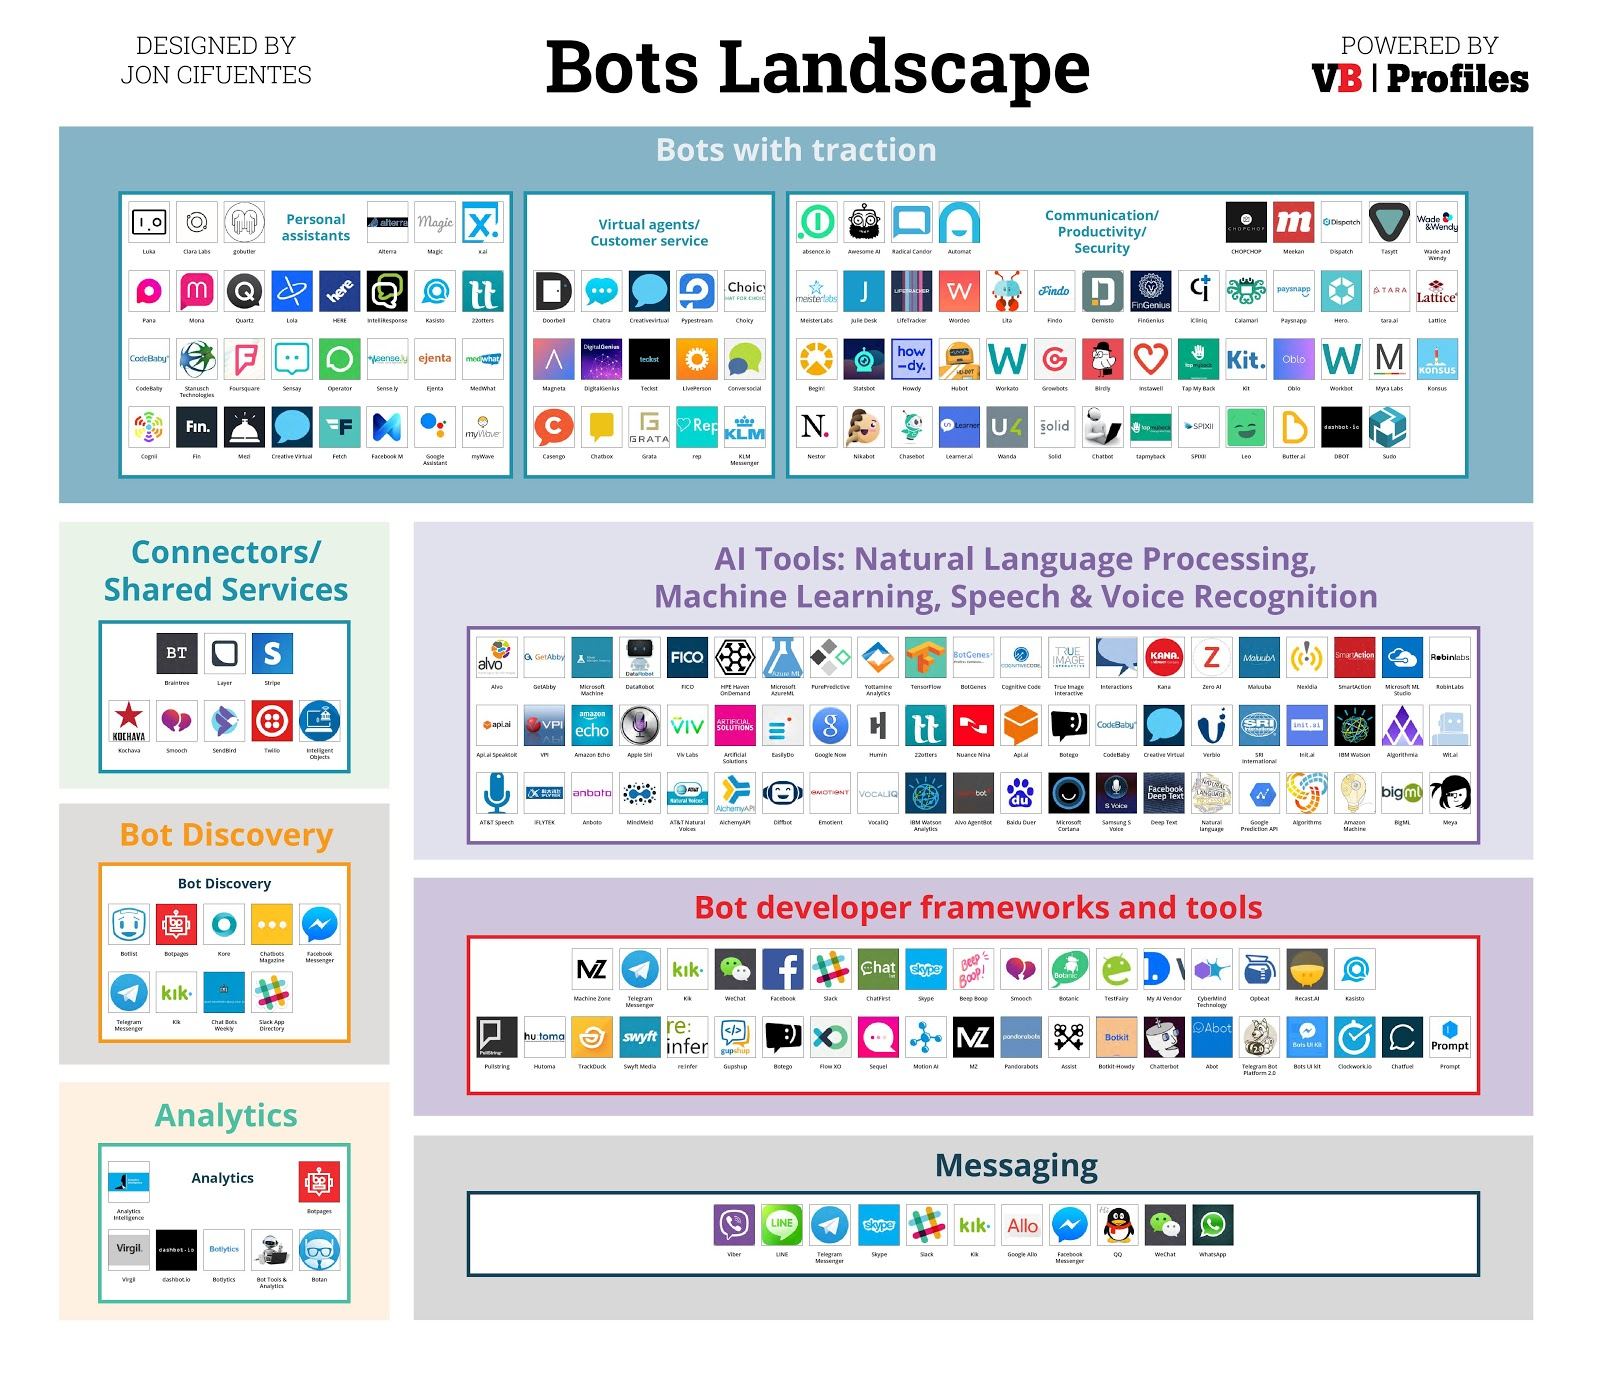
\includegraphics[width=\textwidth]{PanoramaBots.jpg}


\thispagestyle{empty}
\chapter{Conclusiones}

Conluyo que...
\thispagestyle{empty}


%----------------------------------------------------------------------------------------
%	APÉNDICES
%----------------------------------------------------------------------------------------

\addtocontents{toc}{\vspace{2em}} % Agrega espacios en la toc

\appendix % Los siguientes capítulos son apéndices

%  Incluye los apéndices en el folder de apéndices

\chapter{Apéndice}
\section{bot.php}
Código que hace la inserción a CRM
\begin{minted}{php}
<?php
if(isset($_POST['chatfuel'])){
  if($_POST['chatfuel'] == "8cuNbZVtDgYJvkdzYbohnPiY"){
    $_POST['system_id'] = (int)$_POST['system_id'];
    /Translate/
    $_POST['first_name'] = $_POST['fb_first_name']." ".$_POST['fb_last_name'];
    $_POST['phone']     = str_replace(" ","",$_POST['phone']);
    $_POST['phone']     = substr($_POST['phone'],0,10);
    $_POST['landing'] = $_POST['ad_content'];
    $_POST['months_behind'] = str_replace(" meses","",$_POST['meses']);
    $_POST['borrower_insitute'] = $_POST['acredores'];
    $_POST['borrower_insitute'] = $_POST['acredores'];

    /Validation and fix/
    if(!preg_match('/./',$_POST['email'])){
        $_POST['email'] = $_POST['email'].'.com';
    }

    if(filter_var($_POST['email'], FILTER_VALIDATE_EMAIL)) {
    }else{
      $datetime = date("Y_m_d_H_i_s");
      $_POST['email'] = $datetime."@unknown-mail.com";
    }

    function toASCII( $str ){
        return strtr(utf8_decode($str), 
            utf8_decode(
            'ŠŒŽšœžŸ¥µÀÁ ÃÄÅÆÇÈÉÊËÌÍÎÏÐÑÒÓÔÕÖØÙÚÛÜÝßàáâãäåæçèéêëìíîïðñòóôõöøùúûüýÿ'),
            'SOZsozYYuAAAAAAACEEEEIIIIDNOOOOOOUUUUYsaaaaaaaceeeeiiiionoooooouuuuyy');
    }

    $_POST['email']       = toASCII($_POST['email']);
    $_POST['debt_amount'] = str_replace(",","",$_POST['debt_amount']);

    /Unset old values/
    unset($_POST['fb_first_name']);
    unset($_POST['fb_last_name']);
    unset($_POST['ad_content']);
    unset($_POST['meses']);
    unset($_POST['acredores']);
    unset($_POST['chatfuel']);

    /Transform to json/
    $data=json_encode($_POST);
    
    /Test or production/
    $url = 'https://urmdamghr3.execute-api.us-east-1.amazonaws.com/prod/Leads/registerLead';

    $ch = curl_init( $url );
    curl_setopt( $ch, CURLOPT_POST, 1);
    curl_setopt( $ch, CURLOPT_POSTFIELDS, $data);
    curl_setopt( $ch, CURLOPT_FOLLOWLOCATION, 1);
    curl_setopt( $ch, CURLOPT_HEADER, 0);
    curl_setopt( $ch, CURLOPT_RETURNTRANSFER, 1);

    $response = curl_exec( $ch );
  }
}
print_r("v0.3");
exit("");\end{minted}

\section{calculaDescuento.py}
Código que calcula el descuento de los clientes
\begin{minted}[mathescape,gobble=2]{python}
  # coding: utf-8
from __future__ import print_function
import json
import sys
import boto3


print('Loading function')

#event={"institucion": sys.argv[1],"deuda":sys.argv[2],"atraso":sys.argv[3]}
ins=event['institucion']
deuda=round(float((event['deuda'])))
atraso=int(event['atraso'])
descuento=0



def lambda_handler(event, context):    
    """Ejecuta el cálculo del descuento
    Argumentos:
    event -- datos del usuario para cálculo del descuento(dict)
    context --  variables de entorno(str)"""
    print("Parametros recibidos: ")
    print("Institucion= "+ins)
    print("Deuda= " + str(deuda))
    print("Atraso= "+str(atraso))
    
    nuevodescuento=calculaDescuento(ins,atraso)
    print ("Nuevo Descuento="+ str(nuevodescuento))

    nuevadeuda = round(deuda*.01*nuevodescuento)
    print("Nueva deuda="+str(nuevadeuda))
    #nuevadeuda=calculaDescuento(ins,deuda,atraso)
    mensaje1='Tu deuda de $'+ str(deuda)+' con ' +ins+" con atraso de "+ str(atraso)+" meses"
    mensaje2='Quedaria en $'+ str(nuevadeuda)
    print(mensaje1)
    print(mensaje2)

    not_encoded=[{"text": mensaje1},{"text": mensaje2}]
    res=json.dumps(not_encoded)
    
    return(not_encoded)







"""Métodos para calcular descuento
Argumentos:
atraso: meses de atraso(int)"""
descuento=0
def descuentoBancomer(atraso):
    if atraso==1:
            descuento=15
    elif atraso==2:
            descuento=32
    elif atraso==3:
            descuento=48
    elif atraso==4:
            descuento=60
    elif atraso==5:
            descuento=67
    elif atraso>=6:
            descuento=85
    return descuento

def descuentoBanamex(atraso):
    if atraso>=0 and atraso<=4:
        descuento=0
    elif atraso==5:
        descuento=57
    elif atraso==6:
        descuento=62
    elif atraso==7:
        descuento=66
    elif atraso==8 or atraso==9:
        descuento=70
    elif atraso>=6:
        print (str(atraso) +" es mayor a 6")
        descuento=74
        print("entonces descuento="+str(descuento))
    return descuento

def descuentoAmex(atraso):
    if atraso>=0 and atraso<=2:
        descuento=0
    elif atraso==3:
        descuento=5
    elif atraso>=4:
        descuento=25
    return descuento

def descuentoBanorte(atraso):            
    if atraso>=0 and atraso<=4:
        descuento=5
    elif atraso>=5 and atraso<=8:
        descuento=40
    elif atraso>=9:
        descuento=55
    return descuento

def descuentoHSBC(atraso):
    if atraso>=0 and atraso<=2:
        descuento=0,
    elif atraso>=3 and atraso<=4:
        descuento=40,
    elif atraso>=5 and atraso<=6:
        descuento=50,
    elif atraso>6:
        descuento=60
    return descuento

def descuentoScotiabank(atraso):
    if atraso>=0 and atraso<=4:
        descuento=0,
    elif atraso>4:
        descuento=45
    return descuento
def descuentoGlobal(atraso):
    if atraso>=0 and atraso<=4:
        descuento=0
    elif atraso>4:
        descuento=45
    return descuento

def descuentoInbursa(atraso):
    if atraso>=0 and atraso<=4:
        descuento=45
    elif atraso>4:
        descuento=50
    return descuento 



def descuentoCA(atraso):
    if atraso>=1 and  atraso<=4:
        descuento=0
    elif atraso>4:
        descuento=10
    return descuento

def descuentoIxe(atraso):
    if atraso<5:
        descuento=0
    elif atraso>=5:
        descuento=30
    return descuento

def descuentoInvex(atraso):
    if atraso>=0 and atraso<=2:
        descuento=0
    elif atraso==3:
        descuento=35
    elif atraso>=4:
        descuento=45
    return descuento

def descuentoCredFamiliar(atraso):
    if atraso >=1 and atraso<=4: 
        descuento=0
    elif atraso>=5:
        descuento=35
    return descuento

def descuentoSantander(atraso):
    if atraso==1:
         descuento=10
    elif atraso==2:
        descuento=20
    elif atraso==3:
        descuento=30
    elif atraso==4:
        desceunto=50
    elif atraso>=5:
        descuento=55
    return descuento

def descuentoSantander(atraso):
    if atraso==1:
        descuento=10
    elif atraso==2:
        descuento=20
    elif atraso==3:
        descuento=30
    elif atraso==4:
        desceunto=50
    elif atraso>=5:
        descuento=55
    return descuento

def descuentoPH(atraso):
    if atraso>4:
        descuento=15
    return descuento

def descuentoSears(atraso):
    if atraso>4:
        descuento=15
    return descuento

def descuentoCredomatic(atraso):
    if atraso >=1 and atraso<=4:
        descuento=0
    elif atraso>=5 and atraso<=6:
        descuento=10
    elif atraso>6:
        descuento=20
    return descuento

def descuentoWalmart(atraso):
    if atraso>=1 and atraso<=4:
        descuento=0
    elif atraso>=5 and atraso<=6:
        descuento=10
    elif atraso>6:
        descuento=20
    return descuento
def descuentoLiverpool(atraso):
    if atraso>=1 and atraso<=4:
        descuento=0
    elif atraso>=5 and atraso<=6:
        descuento=10
    elif atraso>6:
        descuento=20
    return descuento

def calculaDescuento(ins, atraso):
    """calcula el total a pagar con el descuento
    Argumentos:
    ins -- institucion a la que se le debe(str)
    atraso -- meses pago atrasado(int)"""
    switcher = {
            "Bancomer": descuentoBancomer(atraso),
            "Banamex": descuentoBanamex(atraso),
            "AMEX": descuentoAmex(atraso),
            "Banorte":descuentoBanorte(atraso),
            "HSBC":descuentoHSBC(atraso),
            "Scotiabank":descuentoScotiabank(atraso),
            "Global":descuentoGlobal(atraso),
            "Inbursa":descuentoInbursa(atraso),
            "Liverpool":descuentoLiverpool(atraso),
            "C&A":descuentoCA(atraso),
            "IXE":descuentoIxe(atraso),
            "Invex":descuentoInvex(atraso),
            "Credito Familiar":descuentoCredFamiliar(atraso),
            "Santander":descuentoSantander(atraso),
            "Palacio de Hierro":descuentoPH(atraso),
            "Sears":descuentoSears(atraso),
            "Credomatic":descuentoCredomatic(atraso),
            "Walmart":descuentoWalmart(atraso),
             2: lambda: "two",
    
        }
    func = switcher.get(ins, lambda: "nothing")
    
    # Execute the function
    return func



lambda_handler(event,1)

\end{minted}
\chapter{Imagenes} 
Time Lag - días desde que se produce la primera interacción hasta que se produce la conversión
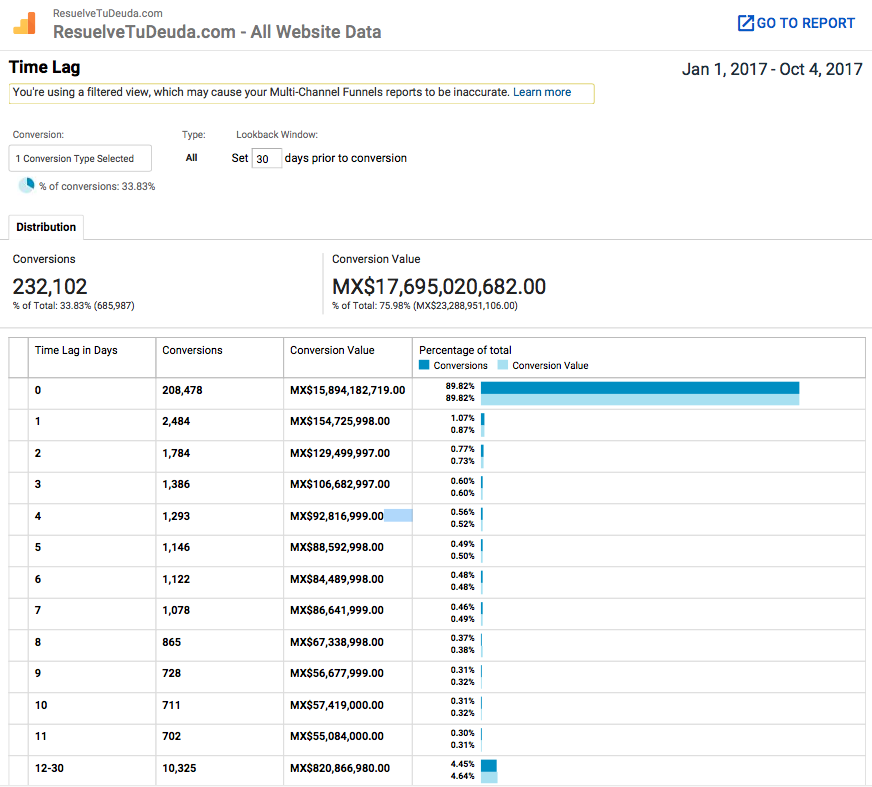
\includegraphics[width=\textwidth]{TimeLag.jpg}

\thispagestyle{empty}
%\include{Apendices/AppendixB}
%\include{Apendices/AppendixC}

\addtocontents{toc}{\vspace{2em}} % Agrega espacio en la toc


%----------------------------------------------------------------------------------------
%	BIBLIOGRAFÍA
%----------------------------------------------------------------------------------------
\backmatter
\nocite{*}
\bibliographystyle{plain}
\bibliography{bibliografía.bib} %Aquí ponen el nombre del archivo .bib






\end{document}